\hypertarget{pm__nonperiodic_8c}{\section{pm\-\_\-nonperiodic.\-c \-File \-Reference}
\label{pm__nonperiodic_8c}\index{pm\-\_\-nonperiodic.\-c@{pm\-\_\-nonperiodic.\-c}}
}


code for non-\/periodic \-F\-F\-T to compute long-\/range \-P\-M force  


{\ttfamily \#include $<$stdio.\-h$>$}\*
{\ttfamily \#include $<$stdlib.\-h$>$}\*
{\ttfamily \#include $<$string.\-h$>$}\*
{\ttfamily \#include $<$math.\-h$>$}\*
{\ttfamily \#include $<$mpi.\-h$>$}\*
\-Include dependency graph for pm\-\_\-nonperiodic.\-c\-:
\nopagebreak
\begin{figure}[H]
\begin{center}
\leavevmode
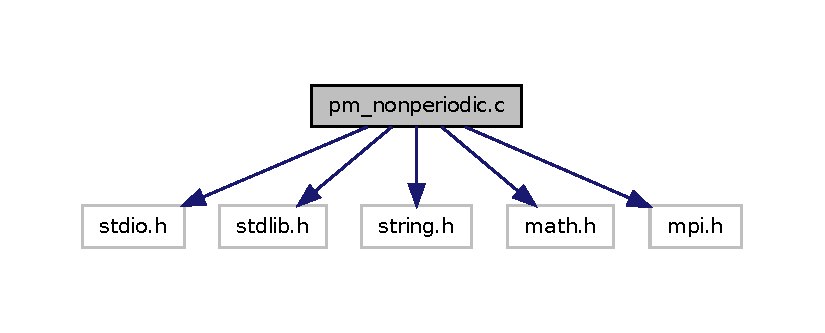
\includegraphics[width=350pt]{pm__nonperiodic_8c__incl}
\end{center}
\end{figure}


\subsection{\-Detailed \-Description}
code for non-\/periodic \-F\-F\-T to compute long-\/range \-P\-M force 

\-Definition in file \hyperlink{pm__nonperiodic_8c_source}{pm\-\_\-nonperiodic.\-c}.

